\section*{Question 6:}
Exercise 9.8:
Cluster the following set of two-dimensional instances into three clusters using each of the five agglomerative clustering methods: 
$$(-4,-2),(-3,-2),(-2,-2),(-1,-2),(1,-1),(1,1),(2,3),(3,2),(3,4),(4,3)$$
Discuss the differences in the clusters across methods. Which methods produce the same clusters? How do these clusters compare to how you would manually cluster the points?

\subsection*{Answer:}

I wrote a simple python script to cluster the data points using each of the five agglomerative clustering methods (single, complete, average, centroid, and ward). The script ``cluster5.py'' clusters the points into 3 clusters. It prints out each point and its cluster number.

\lstinputlisting[language=Python, breakatwhitespace=〈false), label=The content of cluster5.py, caption= The content of cluster5.py]{Q6/cluster5.py}

\begin{lstlisting}[breakatwhitespace=〈false)]
hussam@hussam-HP-Compaq-nc8430-GE542UP-ABA:~/Desktop/A4/Q6$ python cluster5.py
Clustering Method:  single
Cluster:  2 [-4 -2]
Cluster:  2 [-3 -2]
Cluster:  2 [-2 -2]
Cluster:  2 [-1 -2]
Cluster:  3 [ 1 -1]
Cluster:  3 [1 1]
Cluster:  1 [2 3]
Cluster:  1 [3 2]
Cluster:  1 [3 4]
Cluster:  1 [4 3]
Clustering Method:  complete
Cluster:  1 [-4 -2]
Cluster:  1 [-3 -2]
Cluster:  1 [-2 -2]
Cluster:  1 [-1 -2]
Cluster:  2 [ 1 -1]
Cluster:  2 [1 1]
Cluster:  3 [2 3]
Cluster:  3 [3 2]
Cluster:  3 [3 4]
Cluster:  3 [4 3]
Clustering Method:  average
Cluster:  1 [-4 -2]
Cluster:  1 [-3 -2]
Cluster:  1 [-2 -2]
Cluster:  1 [-1 -2]
Cluster:  3 [ 1 -1]
Cluster:  3 [1 1]
Cluster:  2 [2 3]
Cluster:  2 [3 2]
Cluster:  2 [3 4]
Cluster:  2 [4 3]
Clustering Method:  centroid
Cluster:  1 [-4 -2]
Cluster:  1 [-3 -2]
Cluster:  1 [-2 -2]
Cluster:  1 [-1 -2]
Cluster:  3 [ 1 -1]
Cluster:  3 [1 1]
Cluster:  2 [2 3]
Cluster:  2 [3 2]
Cluster:  2 [3 4]
Cluster:  2 [4 3]
Clustering Method:  ward
Cluster:  1 [-4 -2]
Cluster:  1 [-3 -2]
Cluster:  1 [-2 -2]
Cluster:  1 [-1 -2]
Cluster:  3 [ 1 -1]
Cluster:  3 [1 1]
Cluster:  2 [2 3]
Cluster:  2 [3 2]
Cluster:  2 [3 4]
Cluster:  2 [4 3]
Clustering Method:  weighted
Cluster:  1 [-4 -2]
Cluster:  1 [-3 -2]
Cluster:  1 [-2 -2]
Cluster:  1 [-1 -2]
Cluster:  3 [ 1 -1]
Cluster:  3 [1 1]
Cluster:  2 [2 3]
Cluster:  2 [3 2]
Cluster:  2 [3 4]
Cluster:  2 [4 3]
Clustering Method:  median
Cluster:  1 [-4 -2]
Cluster:  1 [-3 -2]
Cluster:  1 [-2 -2]
Cluster:  1 [-1 -2]
Cluster:  3 [ 1 -1]
Cluster:  3 [1 1]
Cluster:  2 [2 3]
Cluster:  2 [3 2]
Cluster:  2 [3 4]
Cluster:  2 [4 3]
hussam@hussam-HP-Compaq-nc8430-GE542UP-ABA:~/Desktop/A4/Q6$
\end{lstlisting}

I used a python library, ``scipy'' to cluster the points. After getting the same results for all 5 clustering methods, I tried two other methods, weighted and median, to see if I get different results, but I did not. Since I am using scipy library as a black box, I was not sure if I am supposed to get the same results. This is how I would manually cluster the points, which is the same result I have from all 7 clustering methods.

\begin{figure}[h]
\caption{Clustering points into 3 clusters}
\centering
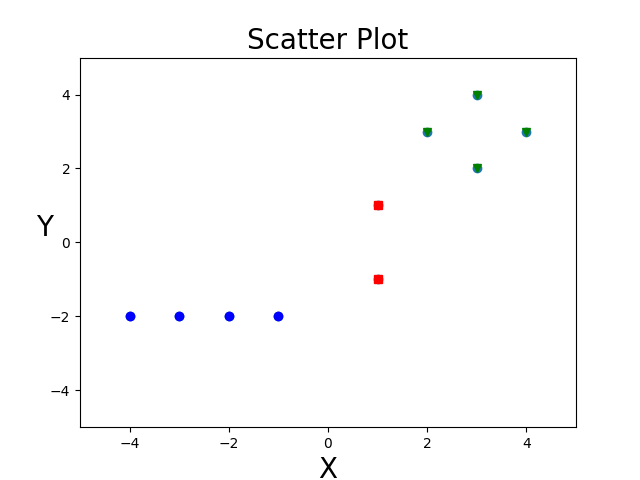
\includegraphics[scale=0.8]{Q6/clusters.png}
\end{figure}
